\chapter{Learning the dictionary}\label{ch:dictionary}

Before CSC-LISTA can train, it needs the atoms $g_m$. The paper's order is the same: learn a dictionary
first, then build the network on top of it, with the dictionary held fixed.

\section{The goal}

Find 32 small atoms, 75 pixels (7.5\um) wide, so that \emph{sharp} simulated fields can be written as
$\sum_m g_m*x_m$ with sparse $x_m$. This stage uses only sharp targets. It never sees the blurred input.

\section{The method: alternate two steps}

Neither the atoms nor the codes are known. So we hold one fixed and improve the other, again and again.

\begin{center}
\begin{tikzpicture}[node distance=6mm and 14mm]
\node[fixed] (crop) {Random sharp crops};
\node[block,right=of crop] (code) {\textbf{Step A}: hold $g$ fixed.\\ Find codes with 30 FISTA steps};
\node[learned,right=of code] (update) {\textbf{Step B}: hold codes fixed.\\ One Adam step on $g$};
\node[block,below=of update] (norm) {Rescale each atom\\ to unit length};
\draw[flow] (crop)--(code); \draw[flow] (code)--(update); \draw[flow] (update)--(norm);
\draw[flow] (norm.west) -| (code.south);
\end{tikzpicture}
\end{center}

\begin{code*}{csc_lista.py}
    for step in range(steps):
        pieces = random_crops(fields, batch, crop, generator, .02).to(device)
        target = torch.nn.functional.pad(pieces, (pad, pad, pad, pad))
        with torch.no_grad():
            x = code_ista(target, Operator(g.data), lam, sparse_steps, pad)
        error = mask * (Operator(g).forward(x) - target)
        loss = .5 * (error ** 2).sum() / batch
        optimiser.zero_grad()
        loss.backward()
        optimiser.step()
        with torch.no_grad():
            g.copy_(unit_norm(g))
\end{code*}

\begin{itemize}
\item \code{code_ista} is FISTA with \code{g} held fixed, and \code{no_grad} means no gradients flow
through it. That is Step A.
\item The \code{error} and \code{loss} lines are Step B, one gradient step on the atoms.
\item \code{unit_norm} rescales each atom to length 1. Without it, atoms could grow and codes could
shrink, which would cheat the $\ell_1$ penalty.
\end{itemize}

The atoms start as real crops of training fields, with the mean removed. Settings: 600 steps, batch 8,
crops of 256 pixels.

\begin{careful}
This procedure is ours. The paper learns its dictionary with Algorithm 1 of Liu et al.\ 2018, which we did
not implement. Alternating sparse coding and gradient steps is a standard idea, but it is a substitute.
\end{careful}

\section{Choosing $\lambda$}

$\lambda$ sets the trade-off between accuracy and sparsity. An early pilot with small $\lambda$ gave codes
that were too dense, so a stronger set was tried. Each dictionary was scored on simulated validation crops,
using 200 FISTA steps.

\begin{center}
\begin{tabular}{ccc}
\toprule
$\lambda$ & Relative $L_2$ of the fit & Density of the codes \\
\midrule
0.1 & 3.2\% & 5.2\% \\
\textbf{0.3} & \textbf{6.4\%} & \textbf{2.4\%} \\
1.0 & 13.8\% & 1.0\% \\
\bottomrule
\end{tabular}
\end{center}

$\lambda=0.3$ was chosen by judgement, as a good balance. The code's automatic rule would have picked
the lowest error, $\lambda=0.1$, but this dictionary was passed in by hand with \code{--dictionary}.

\begin{keyidea}[Why this table is good news]
A fit error of 6.4\% with only 2.4\% of the code values active means 32 atoms really can describe
these fields sparsely. If this had failed, training a network on top would have been pointless.
\end{keyidea}

\section{What the atoms look like}

\begin{figure}[H]
\centering
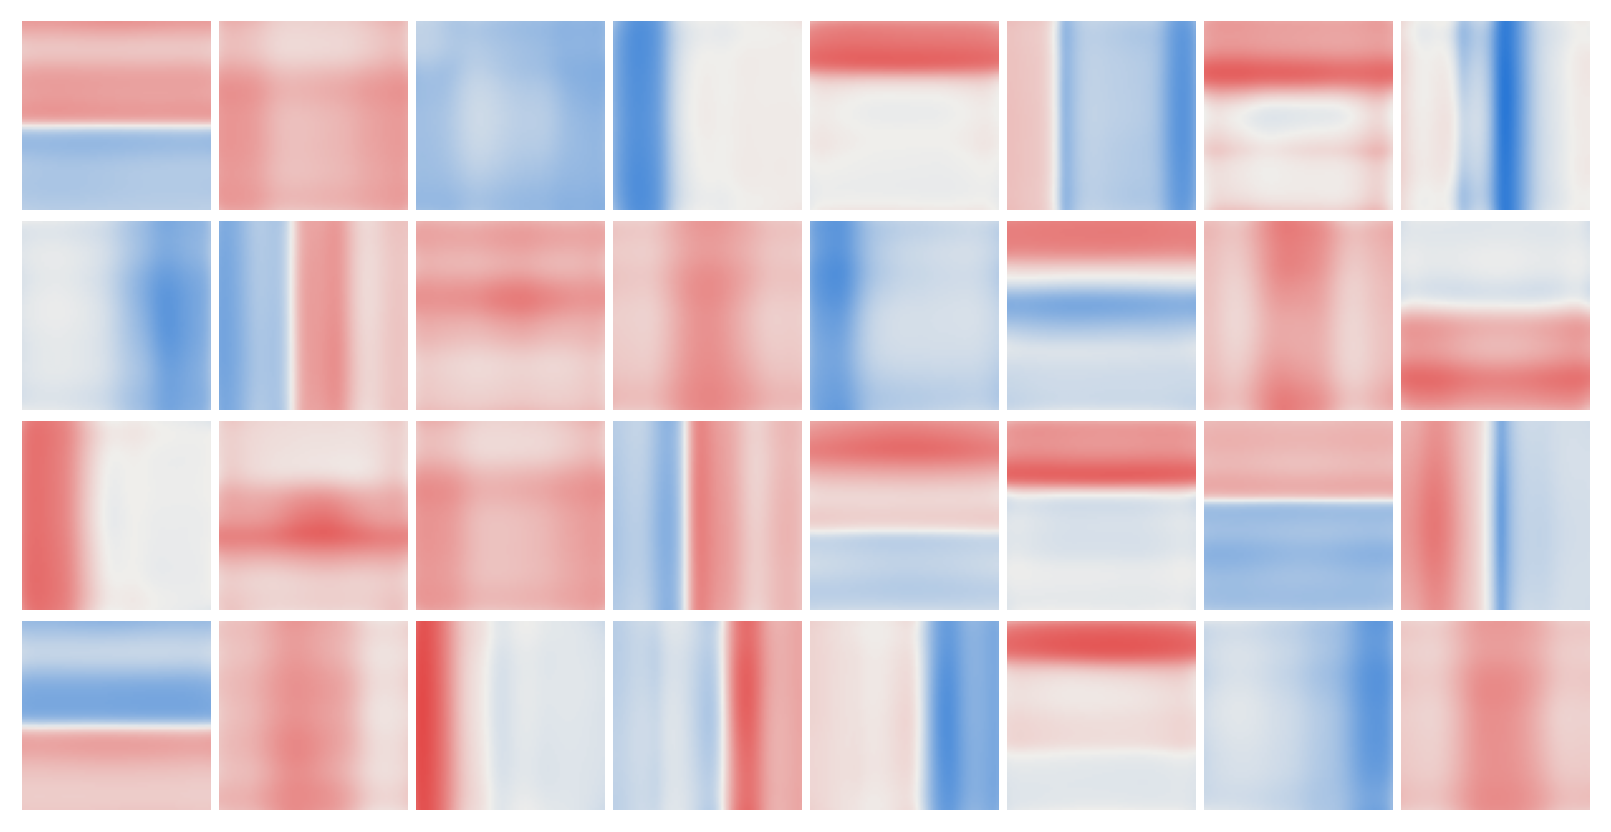
\includegraphics[width=\textwidth]{atoms}
\caption{All 32 learned atoms $g_m$, each 7.5\um\ wide. Red and blue are opposite signs.}
\label{fig:atoms}
\end{figure}

Most atoms in Figure~\ref{fig:atoms} are bars with a sign change. This makes physical sense. The field above
a straight wire has that shape, and our wires are straight segments. The dictionary rediscovered wires from the
data.

\begin{careful}
All three components share one dictionary, and it was trained on the simulated data, so it knows
about Manhattan wires of 1.6--3.2\um. A very different layout would need a new dictionary.
\end{careful}
